\documentclass[12pt, a4paper]{article}
\usepackage[margin=1.25in]{geometry}
\usepackage{graphicx}
\usepackage{amsmath}
\usepackage{float}
\usepackage{listings}
\usepackage{caption}
\usepackage{physics}
\usepackage{mathrsfs}
\usepackage[shortlabels]{enumitem}


\setlength\parindent{0pt}
\newcommand{\code}{\lstinline[basicstyle=\small]}
\lstset{
    language=Python,
    basicstyle=\scriptsize
}


\title{EE2703: Applied Programming Lab \\ \Large Assignment 8: The Digital Fourier Transform}
\author{Soham Roy \\ \normalsize EE20B130}
\date{\today}
\begin{document}

\maketitle % Insert the title, author and date



\section{Introduction}
The goal of this assignment is to analyse signals in the frequency domain. The Discrete Fourier Transform (DFT)
is a powerful tool for this purpose, and has been calculated using the Fast Fourier Transform (FFT) Algorithm.
The Continuous Time Fourier Transform (CTFT) of a gaussian has also been approximated using the FFT. For this,
we use the \code{numpy} library.



\section{Subquestions}

\subsection{Work through the Examples}

\subsubsection{Random Data}
The Fourier Transform of a random signal has been evaluated, and then the Inverse Fourier Transform of
the result is evaluated. The maximum absolute error of the result and the original signal varies, but usually
has an order of magnitude of -16.
\begin{lstlisting}
    x = np.random.rand(100)
    X = fft(x)
    y = ifft(X)
    np.c_[x, y]
    print("Maximum Absolute Error for Random Data: ", np.abs(x - y).max())
\end{lstlisting}

\subsubsection{Spectrum of $\sin(5t)$}
We begin with the following rudimentary code:
\begin{lstlisting}
    x = np.linspace(0, 2 * np.pi, 128)
    y = np.sin(5 * x)
    Y = fft(y)

    plt.figure()
    plt.subplot(2, 1, 1)
    plt.title("Spectrum of $\sin(5t)$ without Phase Wrapping")
    plt.ylabel("$|Y|$")
    plt.plot(np.abs(Y), lw=2)
    plt.grid(True)

    plt.subplot(2, 1, 2)
    plt.xlabel("$\omega$")
    plt.ylabel("Phase of $Y$")
    plt.plot(np.unwrap(np.angle(Y)), lw=2)
    plt.grid(True)
\end{lstlisting}
To obtain:
\begin{figure}[H]
    \centering
    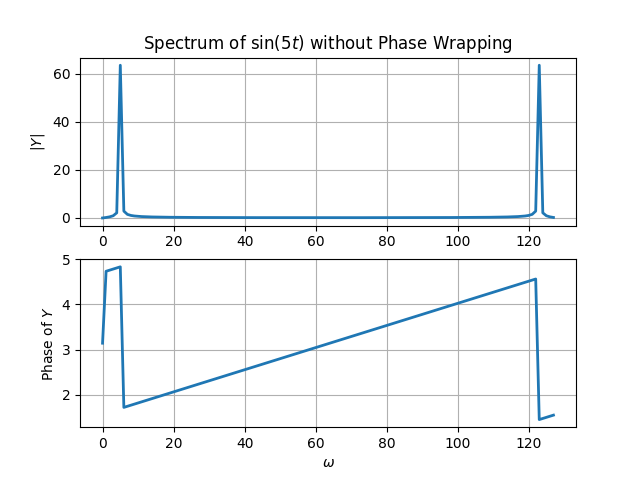
\includegraphics[scale=0.8]{eg1.png}
\end{figure}
The frequencies we sample must exclude $2\pi$, as it is equivalent to 0. The phase plot must also be shifted
to go from $-\pi$ to $\pi$. For this, a helper function \code{plotter()} has also been written.
\begin{lstlisting}
    def plotter(w, Y, title, lim, out, xlabel, ylabels=("$|Y|$", r"$\angle Y$")):
        plt.figure(figsize=(8, 10))
        plt.subplot(2, 1, 1)
        plt.title(title, size=16)
        plt.ylabel(ylabels[0], size=14)
        plt.plot(w, abs(Y), lw=2)
        plt.xlim(-lim, lim)
        plt.grid(True)

        plt.subplot(2, 1, 2)
        plt.xlabel(xlabel, size=14)
        plt.ylabel(ylabels[1], size=14)
        ii = np.where(abs(Y) > 1e-3)
        plt.plot(w[ii], np.unwrap(np.angle(Y[ii])), "go", lw=2)
        plt.xlim(-lim, lim)
        plt.grid(True)

        plt.savefig("Assignment_08/LaTeX/" + out)


    x = np.linspace(0, 2 * np.pi, 128, endpoint=False)
    w = np.linspace(-64, 64, 128, endpoint=False)

    Y = fftshift(fft(np.sin(5 * x))) / 128
    plotter(w, Y, "Spectrum of $\sin(5t)$", 10, "eg2", "$k$")
\end{lstlisting}
\begin{figure}[H]
    \centering
    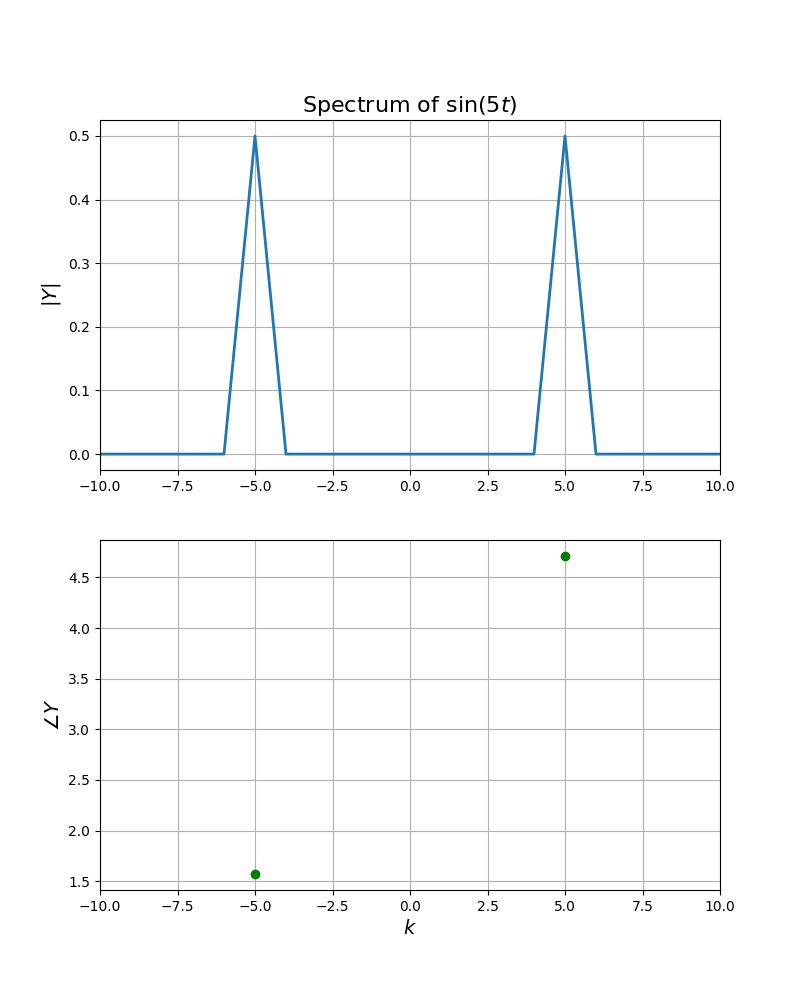
\includegraphics[scale=0.6]{eg2.png}
\end{figure}

\subsubsection{Spectrum of Amplitude Modulated Wave}
The signal to be considered is:
\begin{equation*}
    f(t) = (1 + 0.1\cos(t))\cos(10t)
\end{equation*}
The same helper function has been used as such:
\begin{lstlisting}
    Y = fftshift(fft((1 + 0.1 * np.cos(x)) * np.cos(10 * x))) / 128
    plotter(w, Y, "Spectrum of $(1 + 0.1\cos(t))\cdot\cos(10t)$", 15, "eg3")
\end{lstlisting}
This gives us:
\begin{figure}[H]
    \centering
    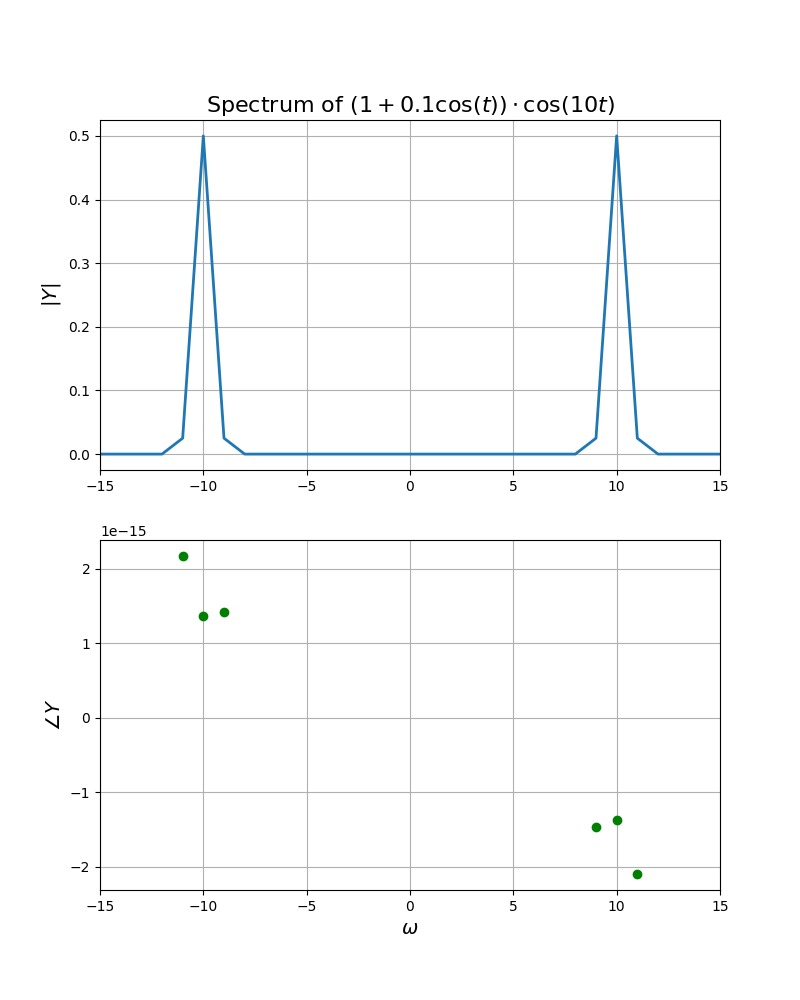
\includegraphics[scale=0.6]{eg3.png}
\end{figure}
The number of samples used is not enough to resolve all the peaks, hence the time vector and the number of
samples have both been increased such that the sampling frequency remains constant.
\begin{lstlisting}
    x = np.linspace(-4 * np.pi, 4 * np.pi, 512, endpoint=False)
    w = np.linspace(-64, 64, 512, endpoint=False)

    Y = fftshift(fft((1 + 0.1 * np.cos(x)) * np.cos(10 * x))) / 512
    plotter(w, Y, "Spectrum of $(1 + 0.1\cos(t))\cdot\cos(10t)$", 15, "eg4")
\end{lstlisting}
Thus, we obtain:
\begin{figure}[H]
    \centering
    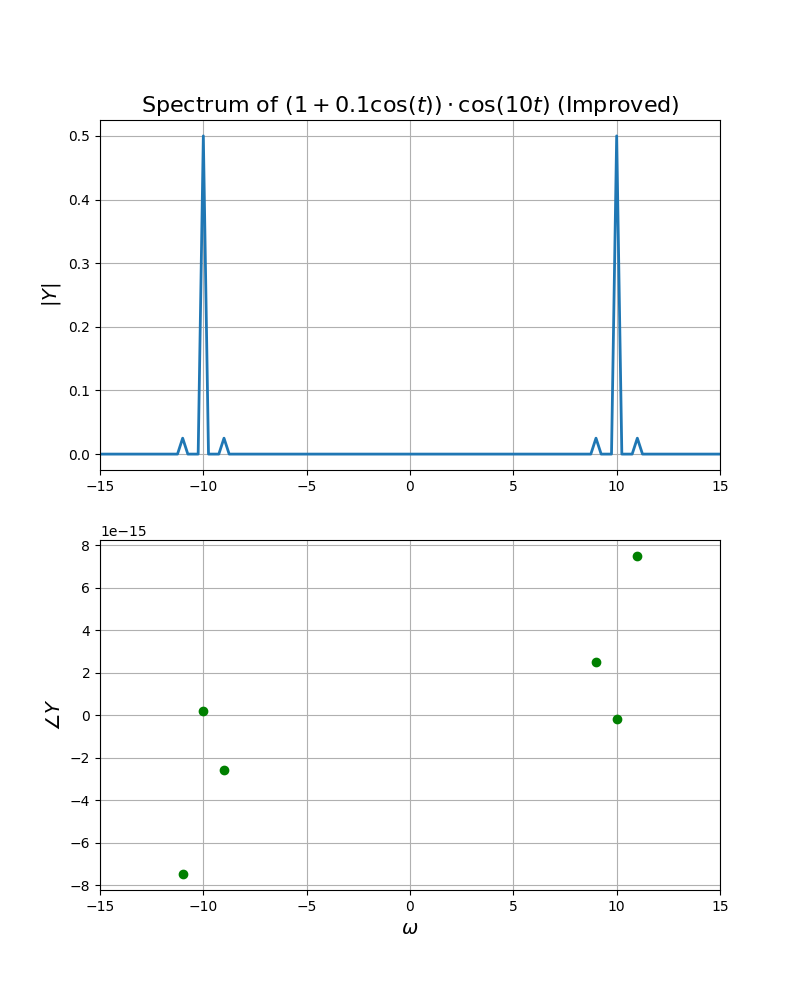
\includegraphics[scale=0.6]{eg4.png}
\end{figure}


\subsection{Generate the Spectrum of $\sin^3(t)$ and $\cos^3(t)$}
\subsubsection{$\sin^3(t)$}
$\sin^3(t)$ can be expressed as a sum of sine waves as:
\begin{equation*}
    \sin^3(t) = \frac{3}{4}\sin(t) - \frac{1}{4}\sin(3t)
\end{equation*}
Thus, 2 peaks are expected: at 1 and 3, with phases being of magnitude $= \frac{\pi}{2}$.
\begin{lstlisting}
    Y = fftshift(fft(np.sin(x) ** 3)) / 512
    plotter(w, Y, "Spectrum of $\sin^3(t)$", 15, "q2a")
\end{lstlisting}
\begin{figure}[H]
    \centering
    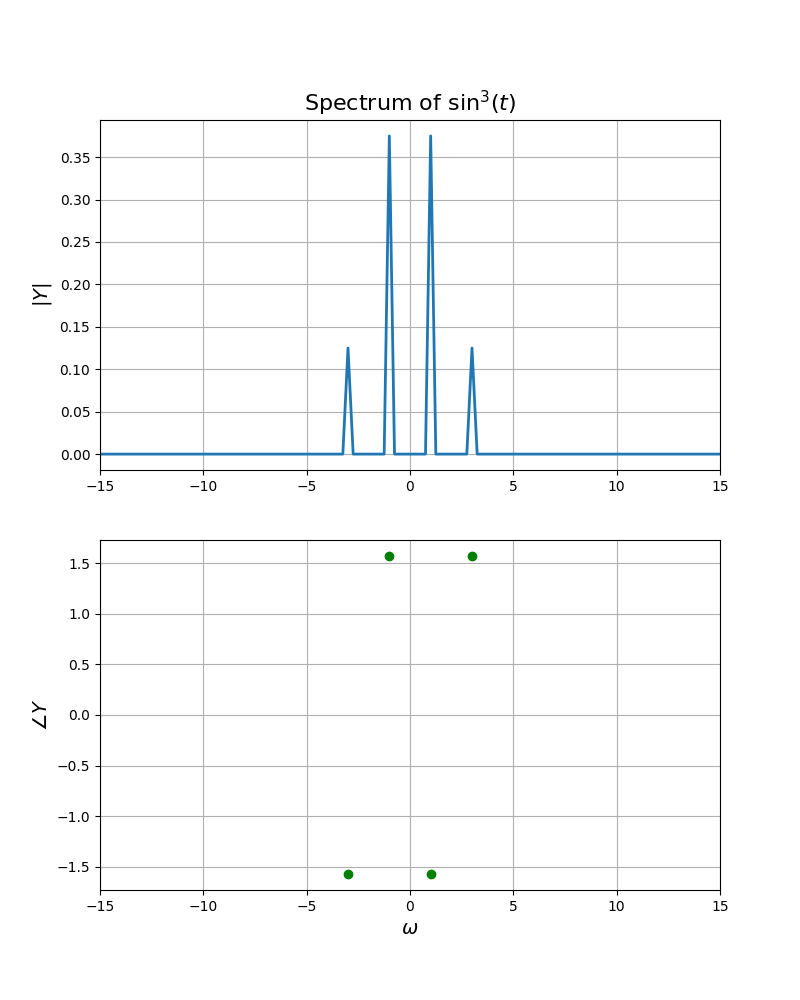
\includegraphics[scale=0.6]{q2a.png}
\end{figure}

\subsubsection{$\cos^3(t)$}
$\cos^3(t)$ can be expressed as a sum of cosine waves as:
\begin{equation*}
    \cos^3(t) = \frac{3}{4}\cos(t) + \frac{1}{4}\cos(3t)
\end{equation*}
Thus, 2 peaks are expected: at 1 and 3, with phases $= 0$.
\begin{lstlisting}
    Y = fftshift(fft(np.cos(x) ** 3)) / 512
    plotter(w, Y, "Spectrum of $\cos^3(t)$", 15, "q2b")
\end{lstlisting}
\begin{figure}[H]
    \centering
    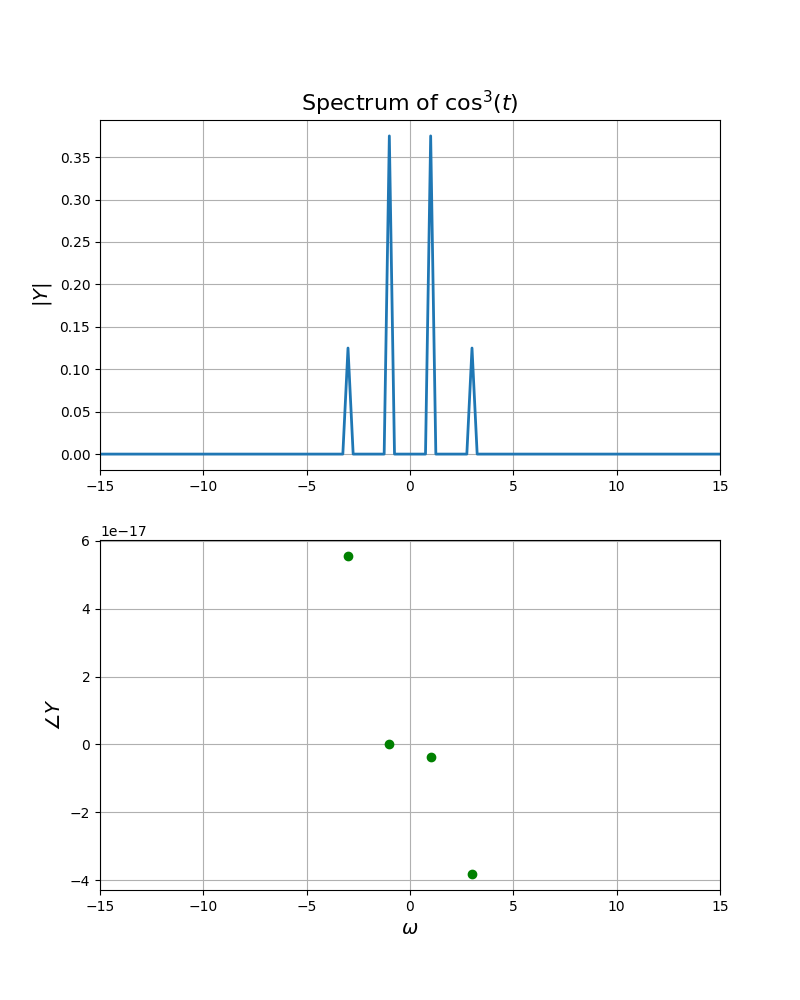
\includegraphics[scale=0.6]{q2b.png}
\end{figure}


\subsection{Frequency Modulated Wave: $\cos(20t + 5\cos(t))$}
The same helper function is invoked as follows:
\begin{lstlisting}
    Y = fftshift(fft(np.cos(20 * x + 5 * np.cos(x)))) / 512
    plotter(w, Y, "Spectrum of $\cos(20t + 5\cos(t))$", 30, "q3")
\end{lstlisting}
This gives us:
\begin{figure}[H]
    \centering
    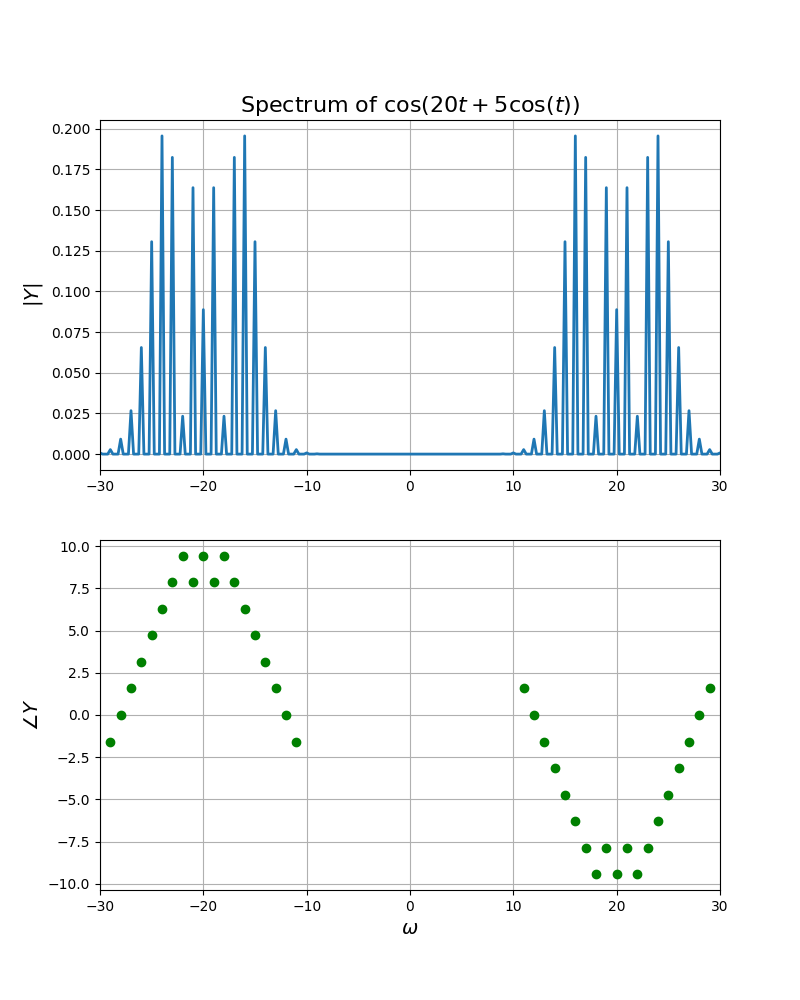
\includegraphics[scale=0.6]{q3.png}
\end{figure}
It can be seen that many more peaks are present, and that single peaks no longer carry a majority of the energy.
Thus, the signal is phase modulated.


\subsection{The Gaussian}
We know that the Fourier Transform of a signal is defined as:
\begin{equation*}
    X(\omega) = \frac{1}{2\pi} \int_{-\infty}^{\infty} x(t) e^{-j\omega t} dt
\end{equation*}
We also know that a Gaussian tends to 0 for large magnitudes of $t$. Thus, for some window size $T$,
we can approximate its Transform as:
\begin{equation*}
    X(\omega) = \frac{1}{2\pi} \int_{-T/2}^{T/2} x(t) e^{-j\omega t} dt
\end{equation*}
Approximating the integral to a Reimann summation of $N$ terms, we get:
\begin{equation*}
    X(\omega) \approx \frac{T}{2\pi N} \sum_{n = -N/2}^{N/2 - 1} x(nT/N) e^{-j\omega nT / N}
\end{equation*}
Where $T / N$ is the time step. Then, let $\omega = 2\pi k / T$:
\begin{equation*}
    X(2\pi k / T) \approx \frac{T}{2\pi N} \sum_{n = -N/2}^{N/2 - 1} x(nT/N) e^{-j2\pi kn/N}
\end{equation*}
We observe that the summation is the Discrete Fourier Transform (DFT) of the signal. Thus, we get:
\begin{equation*}
    X(2\pi k / T) \approx \frac{T}{2\pi N} DFT\{x(nT/N)\}
\end{equation*}
We can improve the accuracy of our obtained approximation by choosing a larger window size while keeping the
sampling frequency constant. We do this iteratively until our error is below a certain threshold.

We compare our approximation to the actual Continuous Time Fourier Transform (CTFT) of the signal:
\begin{equation*}
    \mathscr{F}(e^{-\frac{t^2}{2}}) = \frac{1}{\sqrt{2\pi}}e^{-\frac{\omega^2}{2}}
\end{equation*}

For this, we use the following code:
\begin{lstlisting}
    T = 2 * np.pi
    N = 128
    iter_n = 0
    error = None
    threshold = 1e-6  # 6 decimals of precision

    while error is None or error > threshold:
        t = np.linspace(-T / 2, T / 2, N, endpoint=False)
        w = np.linspace(-np.pi, np.pi, N, endpoint=False) * N / T
        y = np.exp(-0.5 * t ** 2)
        Y = fftshift(fft(ifftshift(y))) * T / (2 * np.pi * N)

        Y_true = np.exp(-0.5 * w ** 2) / np.sqrt(2 * np.pi)
        error = np.sum(np.abs(Y - Y_true))

        T *= 2
        N *= 2
        iter_n += 1
        print(f"Iteration {iter_n}:   Total Error = {error:.2e}")

    T /= 2
    N /= 2

    print(f"Samples = {int(N)},   Time Period = {int(T / np.pi)} pi")

    plotter(w, Y, "Spectrum of Approximated Gaussian", 5, "q4a")
    plotter(w, Y_true, "Spectrum of True Gaussian", 5, "q4b")
\end{lstlisting}
This gives us the graphs:
\begin{figure}[H]
    \centering
    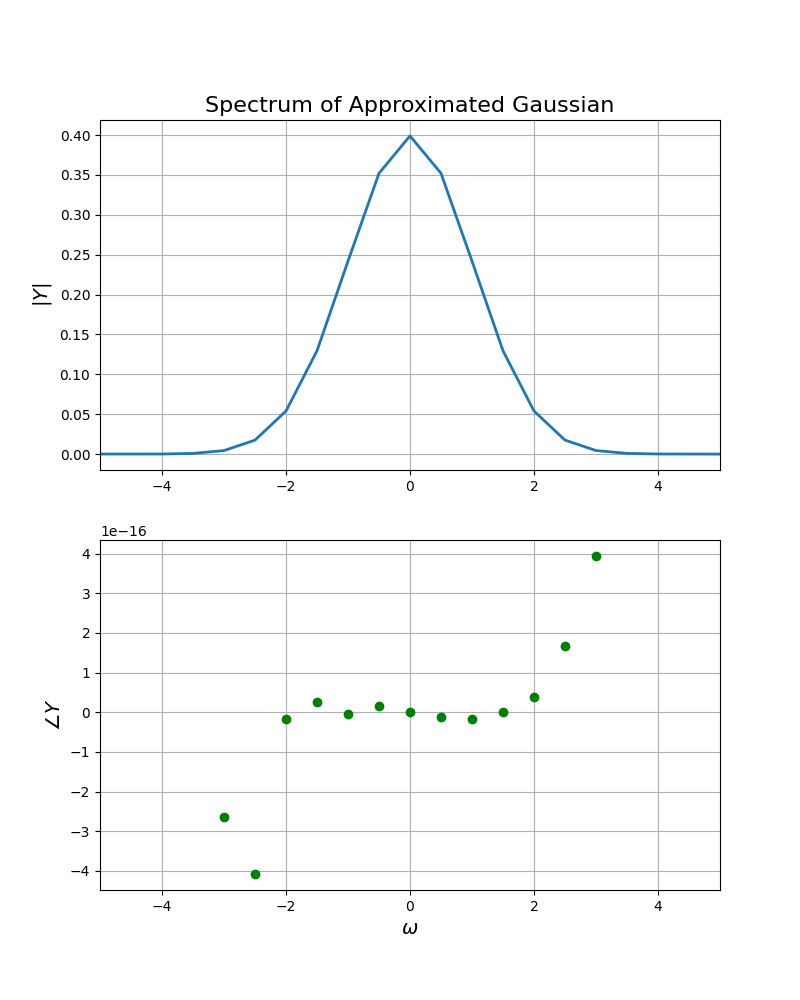
\includegraphics[scale=0.6]{q4a.png}
\end{figure}
Here, we also have the following output:
\begin{lstlisting}
    Iteration 1:   Total Error = 7.19e-03
    Iteration 2:   Total Error = 5.35e-09
    Samples = 256,   Time Period = 4 pi
\end{lstlisting}
Thus, we can say that our approximation converged to an accuracy of 6 decimals very fast.
\pagebreak

To compare, the Continuous Time Fourier Transform results in the following graph:
\begin{figure}[H]
    \centering
    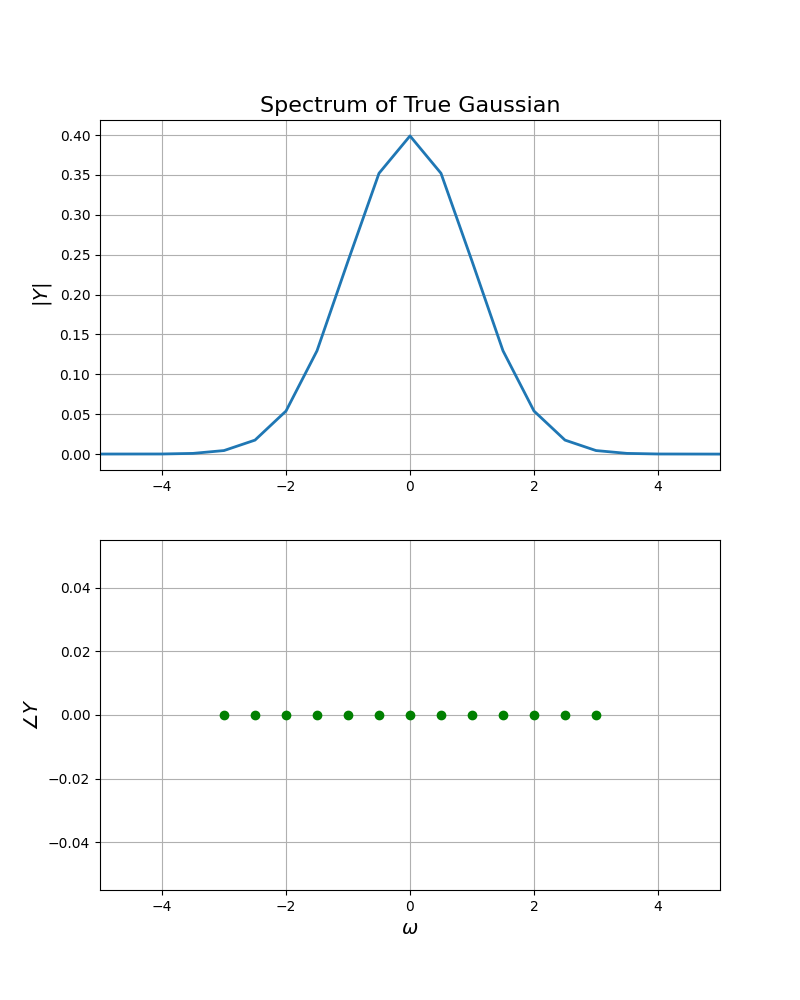
\includegraphics[scale=0.6]{q4b.png}
\end{figure}



\section{Conclusion}
We have calculated the DFT of various signals using the FFT Algorithm. We started with a random signal,
then sinusoids, combinations of sinusoids, and finally a Gaussian.



\end{document}
